\input{src/header}											% bindet Header ein (WICHTIG)
\usepackage{graphicx}
\usepackage{amsmath}
\usepackage{amssymb}
\usepackage{fancyvrb}

\newcommand{\dozent}{Prof. Dr. Margarita Esponda}					% <-- Names des Dozenten eintragen
\newcommand{\tutor}{Lilli Walter}						% <-- Name eurer Tutoriun eintragen
\newcommand{\tutoriumNo}{6}				% <-- Nummer im KVV nachschauen
\newcommand{\projectNo}{5}									% <-- Nummer des Übungszettels
\newcommand{\veranstaltung}{Nichtsequentielle Programmierung}	% <-- Name der Lehrveranstaltung eintragen
\newcommand{\semester}{SoeSe 2017}						% <-- z.B. SoSo 17, WiSe 17/18
\newcommand{\studenten}{Boyan Hristov, Sergelen Gongor}			% <-- Hier eure Namen eintragen
% /////////////////////// BEGIN DOKUMENT /////////////////////////


\begin{document}
% /////////////////////// BEGIN TITLEPAGE /////////////////////////
\begin{titlepage}
	\subject{\dozent}
	\title{\veranstaltung, \semester}
	\subtitle{\Large Übungsblatt \projectNo\\ \large\vspace{1ex} }
	\author{\studenten}
	\date{\normalsize \today}
\end{titlepage}

\maketitle								% Erstellt das Titelblatt
\vspace*{-9cm}							% rückt Logo an den oberen Seitenrand
\makebox[\dimexpr\textwidth+1cm][r]{	%rechtsbündig und geht rechts 1cm über Layout hinaus
	\includegraphics[width=0.4\textwidth]{src/fu_logo} % fügt FU-Logo ein
}
% /////////////////////// END TITLEPAGE /////////////////////////

\vspace{7cm}							% Abstand
\rule{\linewidth}{0.8pt}				% horizontale Linie										% erstellt die Titelseite


Link zum Git Repository: \url{https://github.com/BoyanH/FU-Berlin-ALP4/tree/master/Solutions/Homework5}

% /////////////////////// Aufgabe 1 /////////////////////////

\section*{1. Aufgabe}

\begin{enumerate}
    
\item[a)]
Um diese Aufgabe richtig zu beantworten, muss man Annahme über welche Threads zu erst bei dem Scheduling-Algorithmus ankommt, obwohl die alle gleich gestartet werden. Das liegt daran, dass bei nicht prämptive Algorithmen ein Thread nie unterbrochen wird, bevor dieser zu Ende ausgeführt wurde.

\begin{enumerate}

\item[1. ] nicht-präemptive FCFS \\ \\
Hier machen wir die Annahme, dass der Thread mit 100 Minuten Ausführungszeit erster ankommt. So unterscheiden sich auch die erste 2 Teilaufgaben \\ \\
Gesammte Ausführungszeit = $100 + 100 \times 1 = 200$ \\ \\
Durchschnittliche Ausführungszeit = $ \frac{200}{101} \approx $ 1,98 Minuten \\ \\
Gesammte Wartezeit = $0 + 99 \times 100 + \sum_{i=0}^{99} i = 990 + \frac{99(99+1)}{2} = \frac{1999}{2}$ \\ \\
Durchschnittliche Wartezeit = $\frac{1999}{2 \times 101} = \frac{1999}{202} \approx $ 9,896 Minuten \\ \\
Damit durchschnittliche Verarbeitungszeit = $\frac{200 + \frac{1999}{2}}{101} \approx $ 11,876 Minuten \\

\item[2. ] nicht-präemptive SJF \\ \\
Gesammte Ausführungszeit = $100 \times 1 + 100 = 200$ \\ \\
Durchschnittliche Ausführungszeit = $ \frac{200}{101} \approx $ 1,98 Minuten \\ \\
Gesammte Wartezeit = $(\sum_{i=0}^{99} i) + 100 = \frac{199}{2} + 100 =  $ 199,5 Minuten \\ \\
Durchschnittliche Wartezeit = $\frac{199.5}{101} \approx $ 1,975 Minuten \\ \\
Damit durchschnittliche Verarbeitungszeit = $\frac{199,5 + 200}{101} \approx $ 3,955 Minuten \\

Unter der Annahme, dass 1. Thread mit 100 Minuten Ausführungszeit als 1. gescheduled wird bekommt man das Ergebniss von FCFS. Wir gehen aber davon aus, dass der Scheduling-Algorithmus schon alle Threads kennt.

\item[3. ] präemptive Shortest Remaining Time First. Quantum = 1 Minute \\
Da hier alle Threads gleichzeitig gestartet werden, gehen wir auch davon aus, dass diese in der selben Reihenfolge zu dem Scheduler ankommen. Da alle gleich gestartet werden un keine Threads mit kürzerer Ausführungszeit inzwischen kommen, ist die Ausführung analog zu diese von nicht-präemptive SJF. \\

Man kann hier die Annahme machen, dass 1. Thread mit Ausführungszeit von 100 Minuten als erster gescheduled wird und dann unterbrochen wird, dann kommt man bei dem Ergebniss von RR. Wie vorher, ist unsere Annahme, dass der Scheduler schon alle Threads kennt. \\

Durchschnittliche Wartezeit = $\frac{199.5}{101} \approx $ 1,975 Minuten \\ \\
Durchschnittliche Verarbeitungszeit $\approx$ 3,96 Minuten \\ 

\item[4. ] RR-Scheduling. Quantum = 1 Minute \\
Bei Quantum gleich eine Minute werden alle Threads mit kleine Anforderungen gleich auf der ersten Runde ausgeführt und am Ende bleibt nur das eine Thread noch laufen. Um die Berechnung interessanter zu machen gehen wir davon aus, dass der Thread mit 100 Minuten Ausführungszeit als erster gestartet wurde.\\ \\
%
Gesammte Ausführungszeit = Ausführungszeit für 1. Thread + Ausführungszeit für restliche 100 Threads + Restausführungszeit für 1. Thread = \\
= $1 + (100 \times 1) + 99 = 200 $ \\ \\
Durchschnittliche Ausführungszeit = $\frac{200}{101} \approx $ 1,98 Minuten \\ \\
Gesammte Wartezeit = Initiale Wartezeit für 1. Thread (0) + Wartezeiten für einzelne Threads mit Ausführungszeit 1 + Wartezeit für 1. Thread = \\
= $ 0 + (\sum_{i=1}^{100} i) + 100 =  \frac{201}{2} + 100 =  $ 199,5 Minuten \\ \\
Durchschnittliche Wartezeit = $\frac{200,5}{101} \approx $ 1,985 Minuten \\ \\
Durchschnittliche Verarbeitungszeit = $\frac{200,5 + 200}{101} \approx $ 3,965 Minuten 


\end{enumerate}

\item[b)]
Nicht-prämptive FCFS ist ein sehr simpler Algorithmus mit geringsten Overhead. Der ist gut für Scheduling von unabhängige, gleich große Aufgaben, die erst dann fertig sind, wenn alle fertig sind. Z.B. bei Verarbeitung und Analyse von Daten an einem Server.

Nicht-präemptive SJF ist besser für Scheduling von unterschiedlich-aufwändige Aufgaben, wo wir relativ sicher sind, dass keine neue Aufgaben inzwischen kommen. Der Algorithmus ist wieder aufwändbar für Bearbeitung von schon am Anfang bekannte Jobs. Diser Algorithmus funktioniert aber wesentlich besser für Jobs mit unterschiedliche Ausführungszeit.

Präemptive Shortest Remaining Time First ist schon deutlich besser für simple Betriebssysteme. Hier können Jobs mit unterschiedliche Aufforderungen gut behandelt werden, neu gekommene Threads mit kurze Ausführungszeiten müssen nicht lange warten. 

Mit Round-Robin kann man aber deutlich besser Scheduler für Threads mit unbekannte Ausführungszeiten bauen. Das liegt daran, dass jeden Thread eien feste Zeitfenster kriegt, in dem dieser fertig sein soll, sonst wartet er auf die nächste Runde. Der Algorithmus eignet sich gut für Systemen, wo Ausführungszeit von einzelne Threads schwer zu schätzen ist.

\end{enumerate}

\section*{2. Aufgabe}

\begin{enumerate}

\item[a)]
FCFS - Es könnte sein, dass einige Threads lange auf den aufwändigen Threads vor denen warten, die werden aber alle irgendwann ausgeführt, da der Algorithmus mit einer Schlange funktioniert.

\item[b)]
SJF - Hier können aufwändigere Threads sehr leicht verhungern, in dem immer wieder neue Threads kommen mit sehr geringe Ausführungszeit.

\item[c)]
RR - hier könnte es wieder sein, dass einige Threads mit längeren Ausführungszeiten mehrmals gestartet / weiter ausgeführt werden bevor diese fertig werden, Threads werden aber nicht verhungern.

\item[d)]
O(1) früheres Linux-Scheduling - Threads mit geringere Priorität haben nur halb so große Quantums, es könnte wieder sein dass einige deutlich länger verarbeitet werden, Threads verhungern aber wieder nicht.

\item[e)]
Hybrid Lottery Scheduling - da alle Prozesse eine Mindestanzahl von Losen haben, verhungern keine Prozesse / Threads.

\item[f)]
Completely Fair Scheduling - die Frage kann mit Argumente aus der Vorlesung leider nicht beantwortet werden. Der Fair Scheduler benutzt aber die Zeit, in dem ein Prozess zu der Scheduler gekommen ist, als auch die letzte Ausführungszeit um die Prioritäten von ältere Prozessen zu erhöhen, vermeidet so erfolgreich das Verhungern von Prozessen.

Quelle $\rightarrow$ \url{https://stackoverflow.com/questions/39725102}

\end{enumerate}

\section*{3. Aufgabe}

Die Bilder kann man in GitHub besser anschauen

\begin{enumerate}

\item[a)] RMS \\
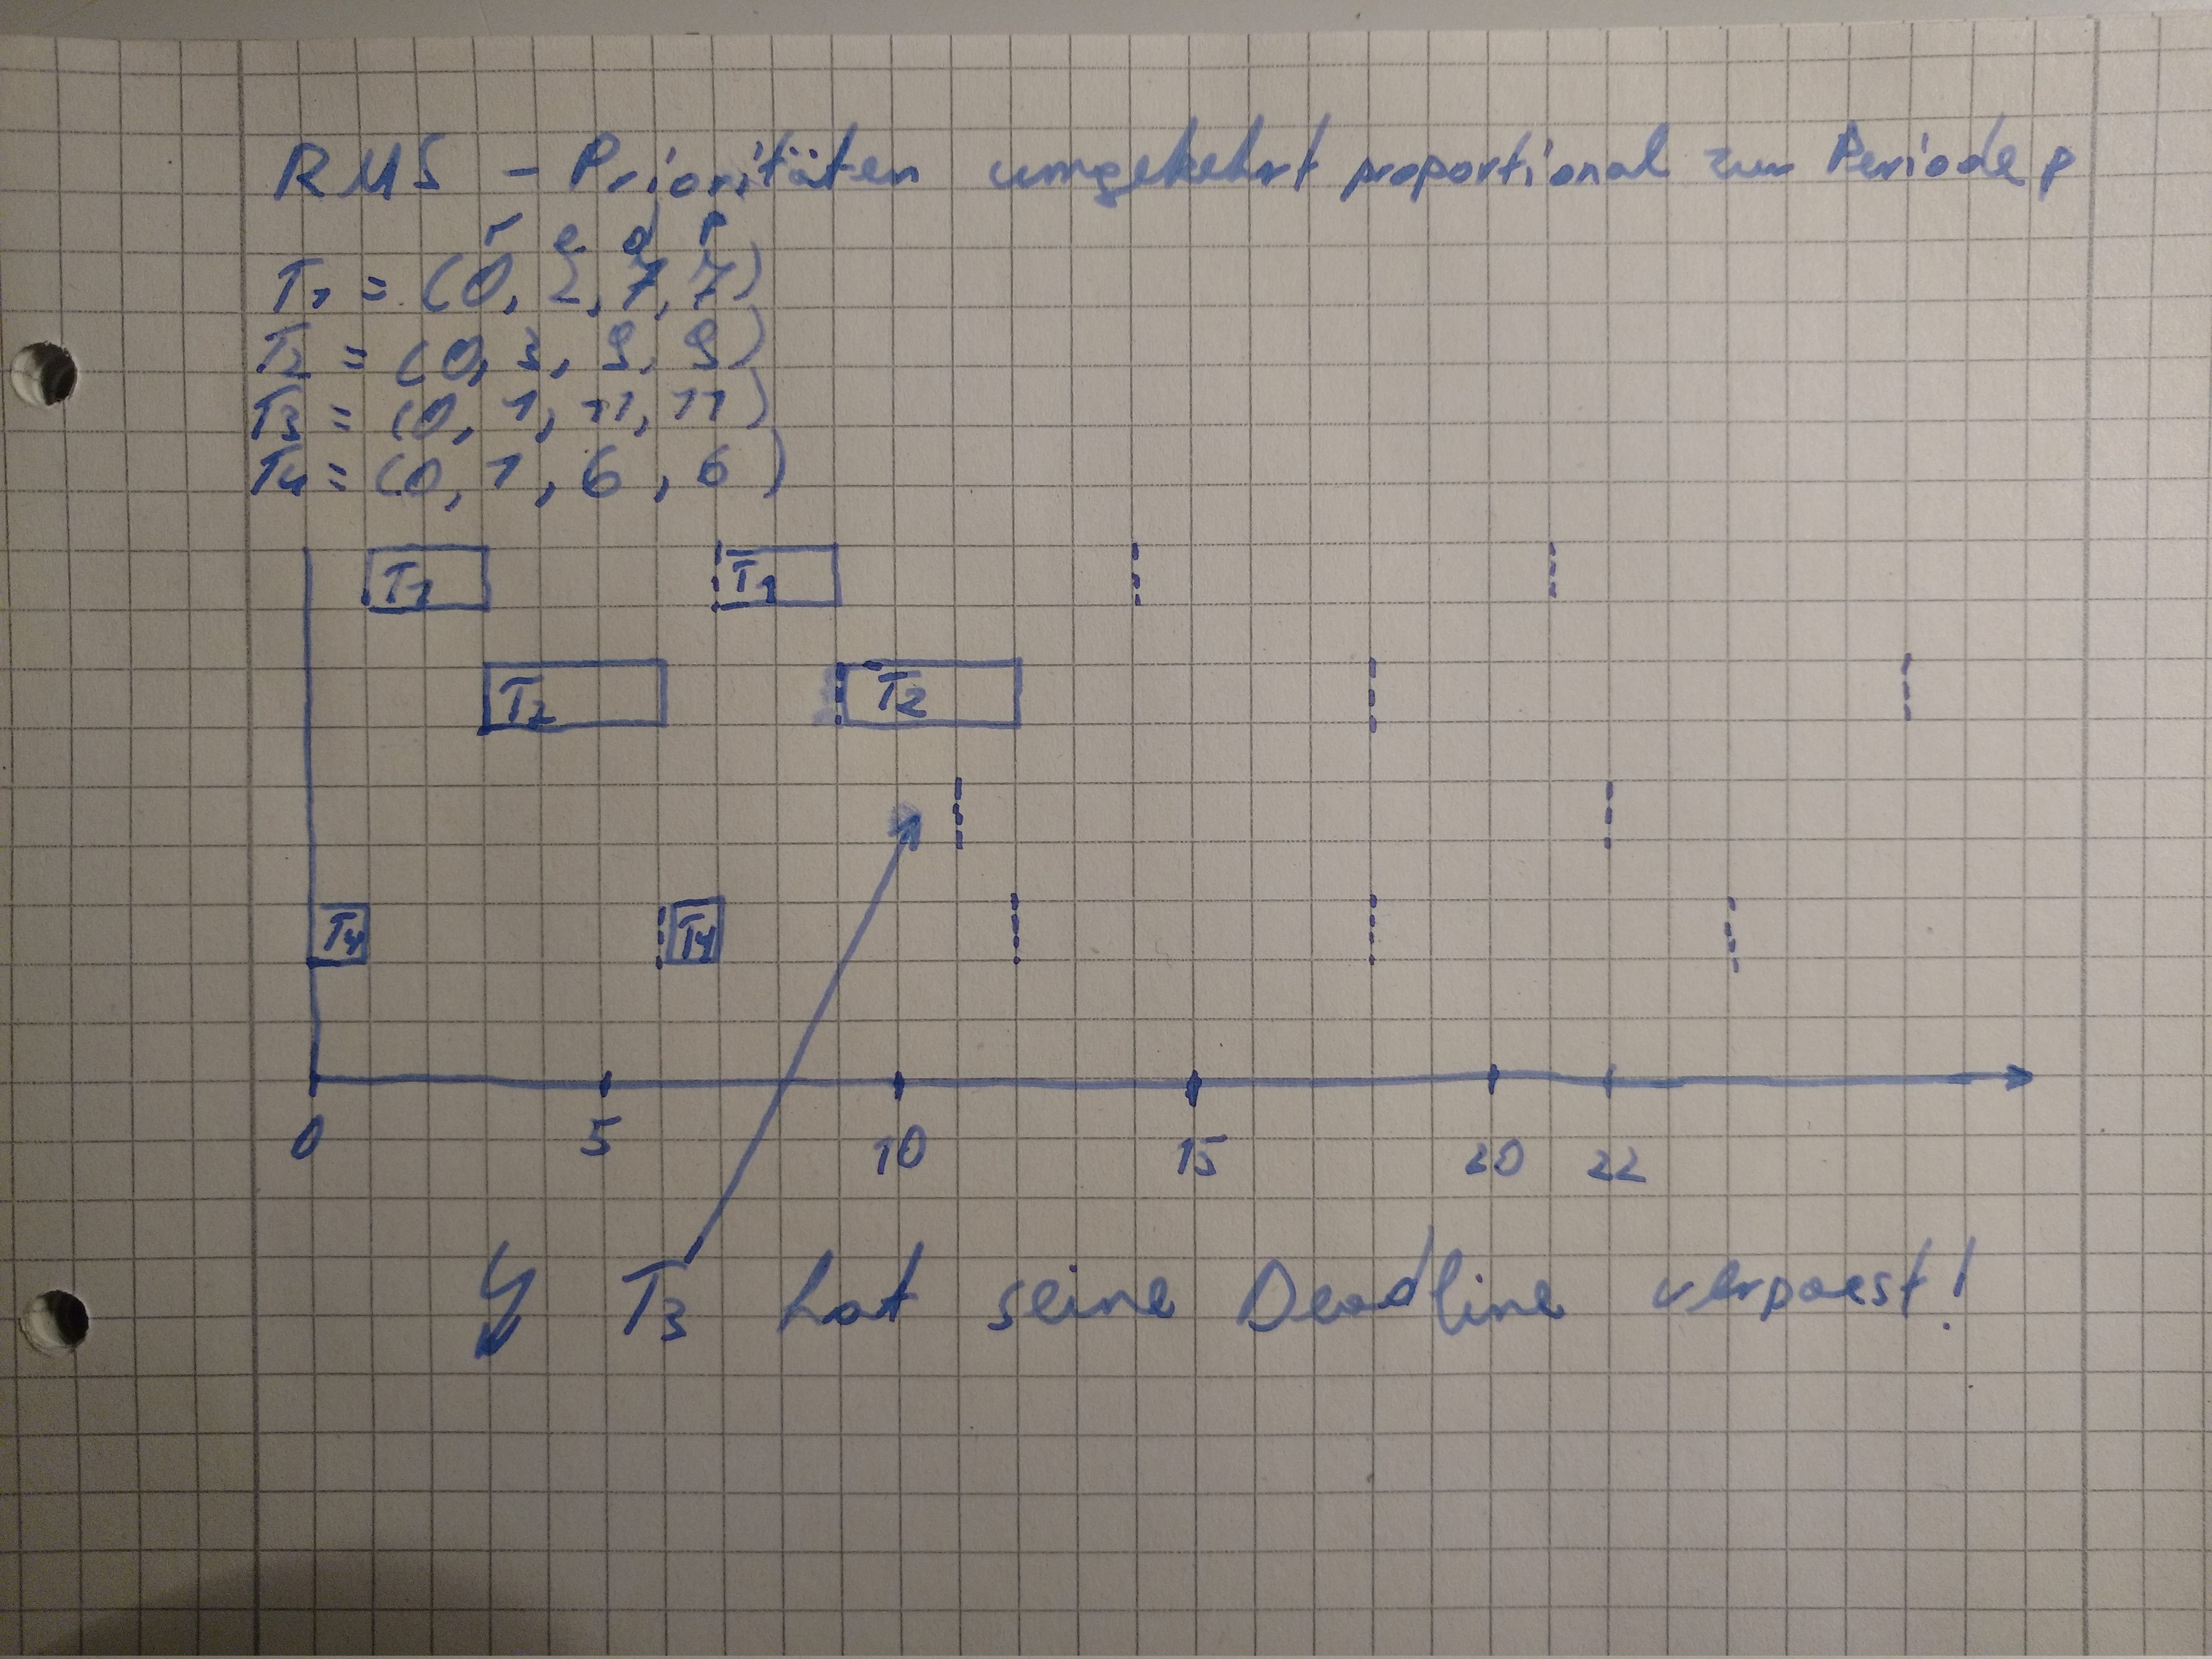
\includegraphics[width=\textwidth]{./exercise3/RMS.jpg} \clearpage
\item[b)] DMS \\
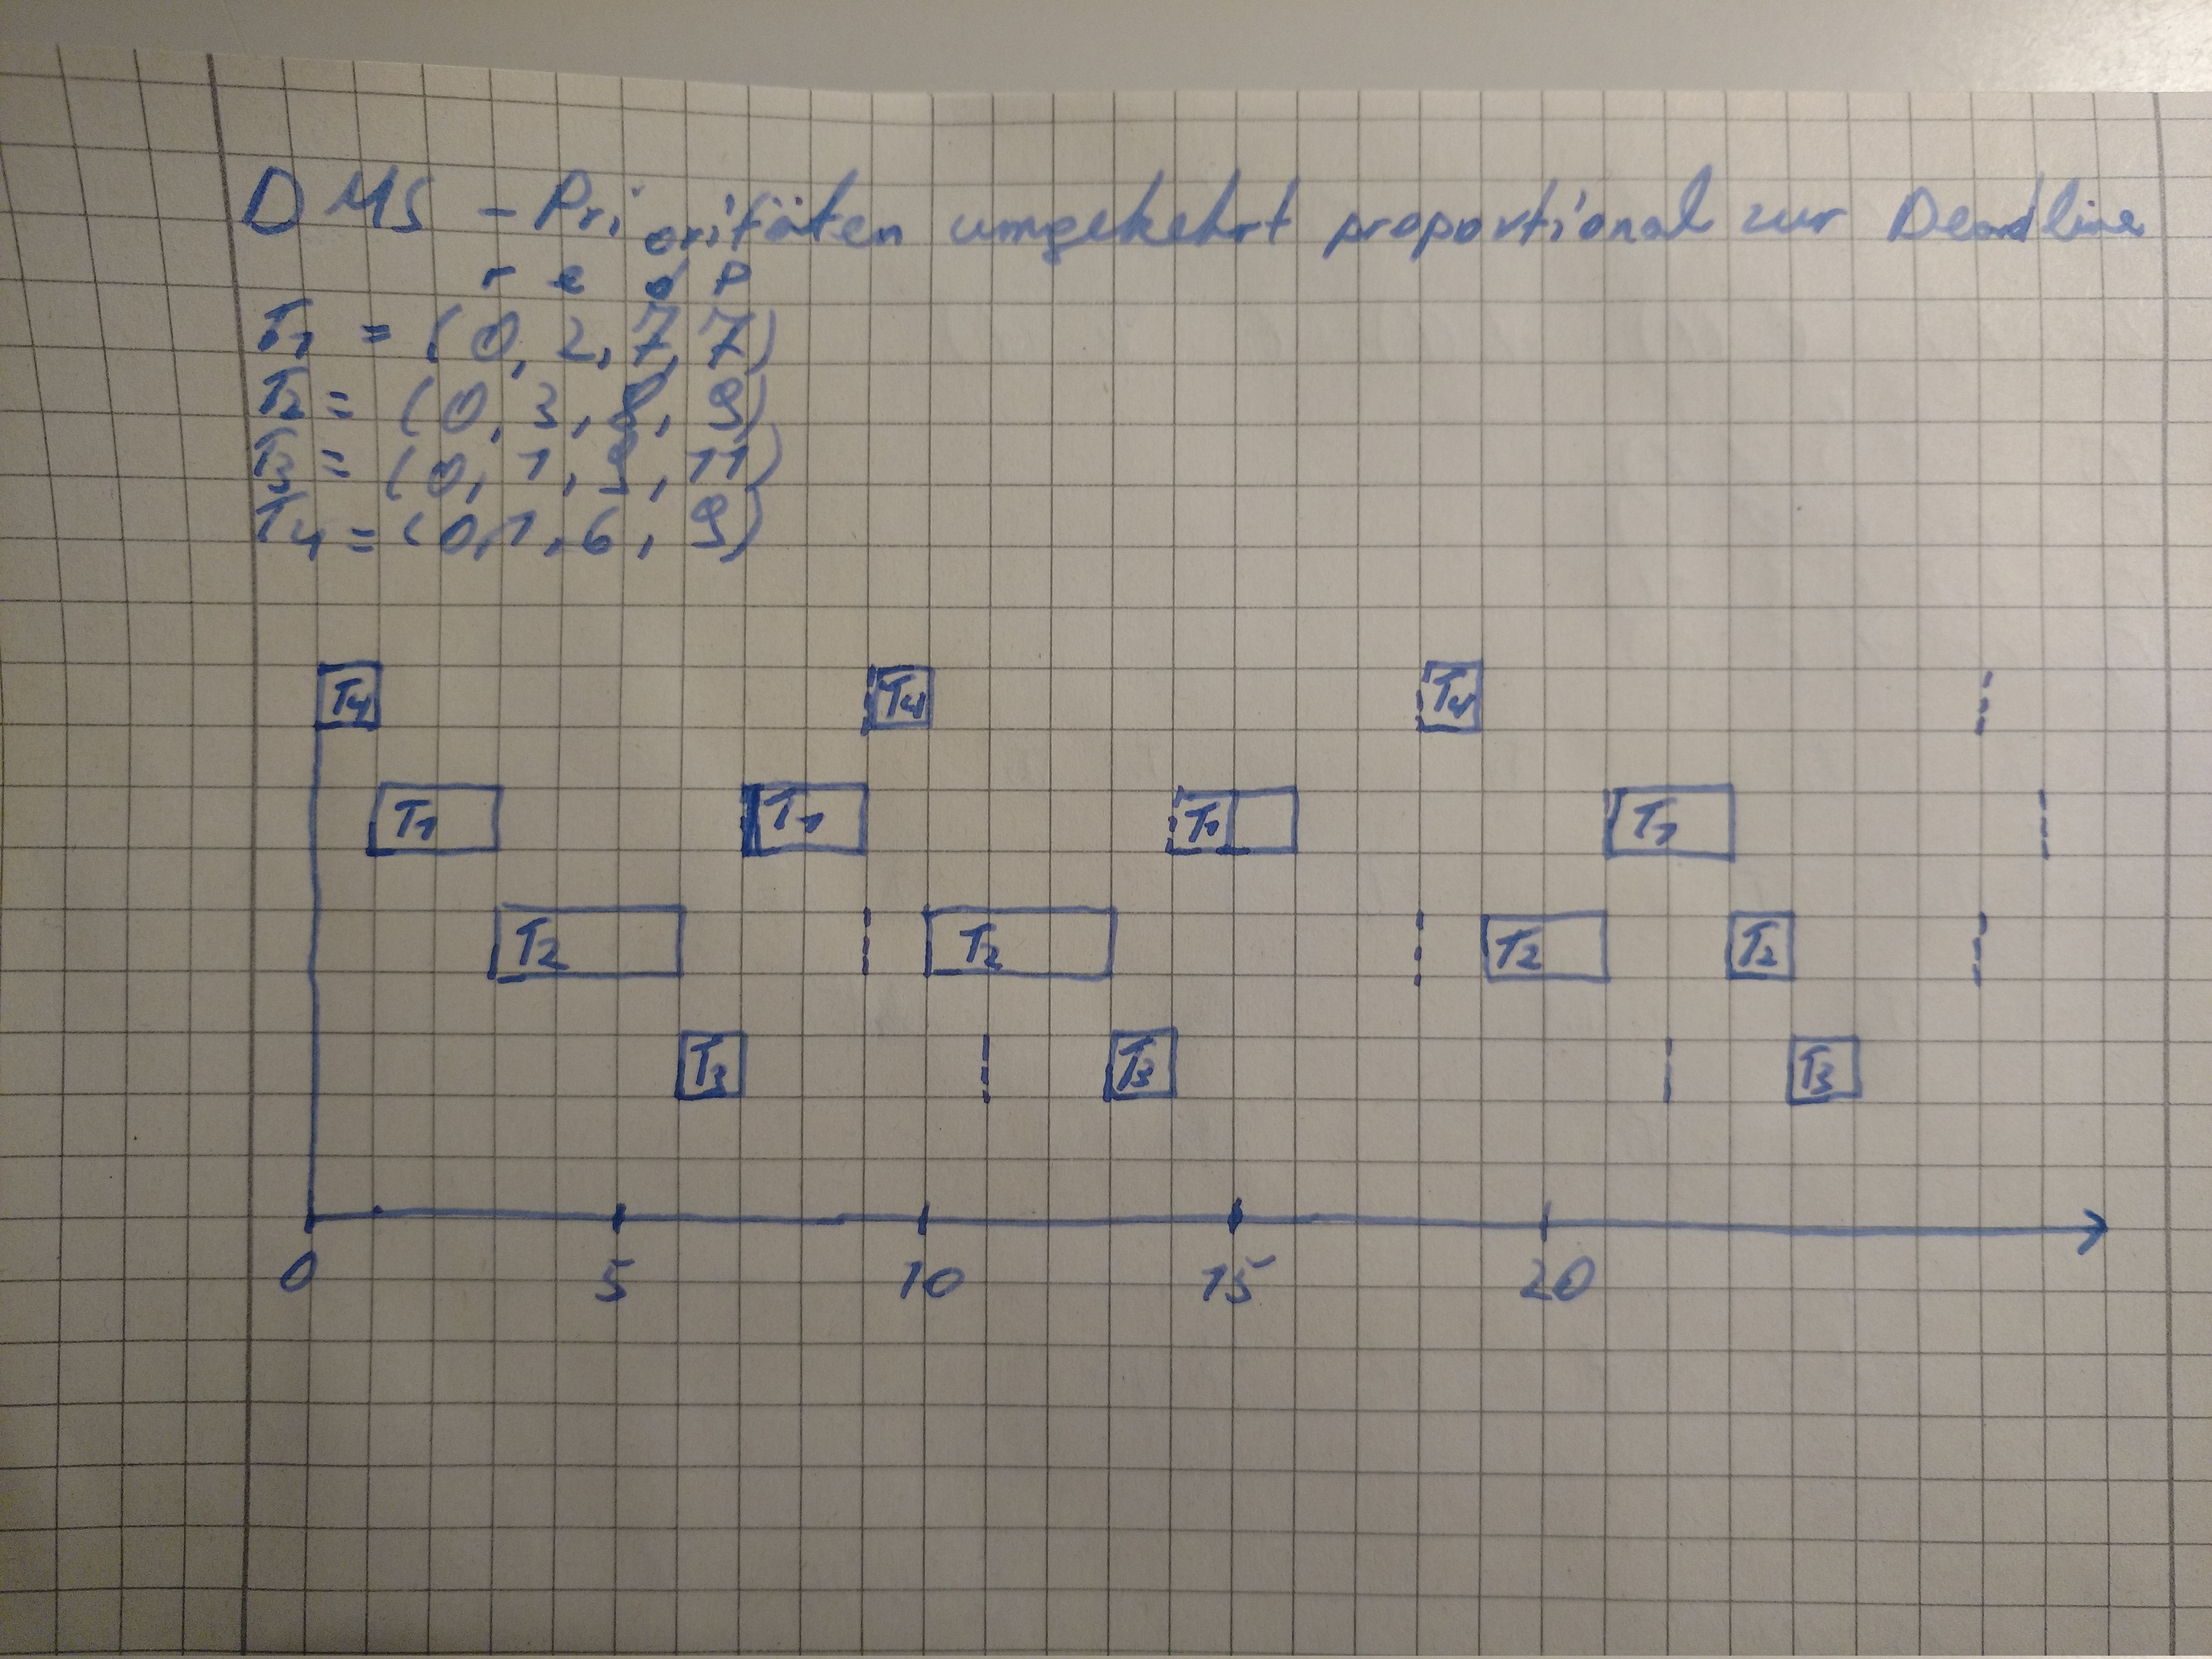
\includegraphics[width=\textwidth]{./exercise3/DMS.jpg} \clearpage
\item[c)] EDF \\
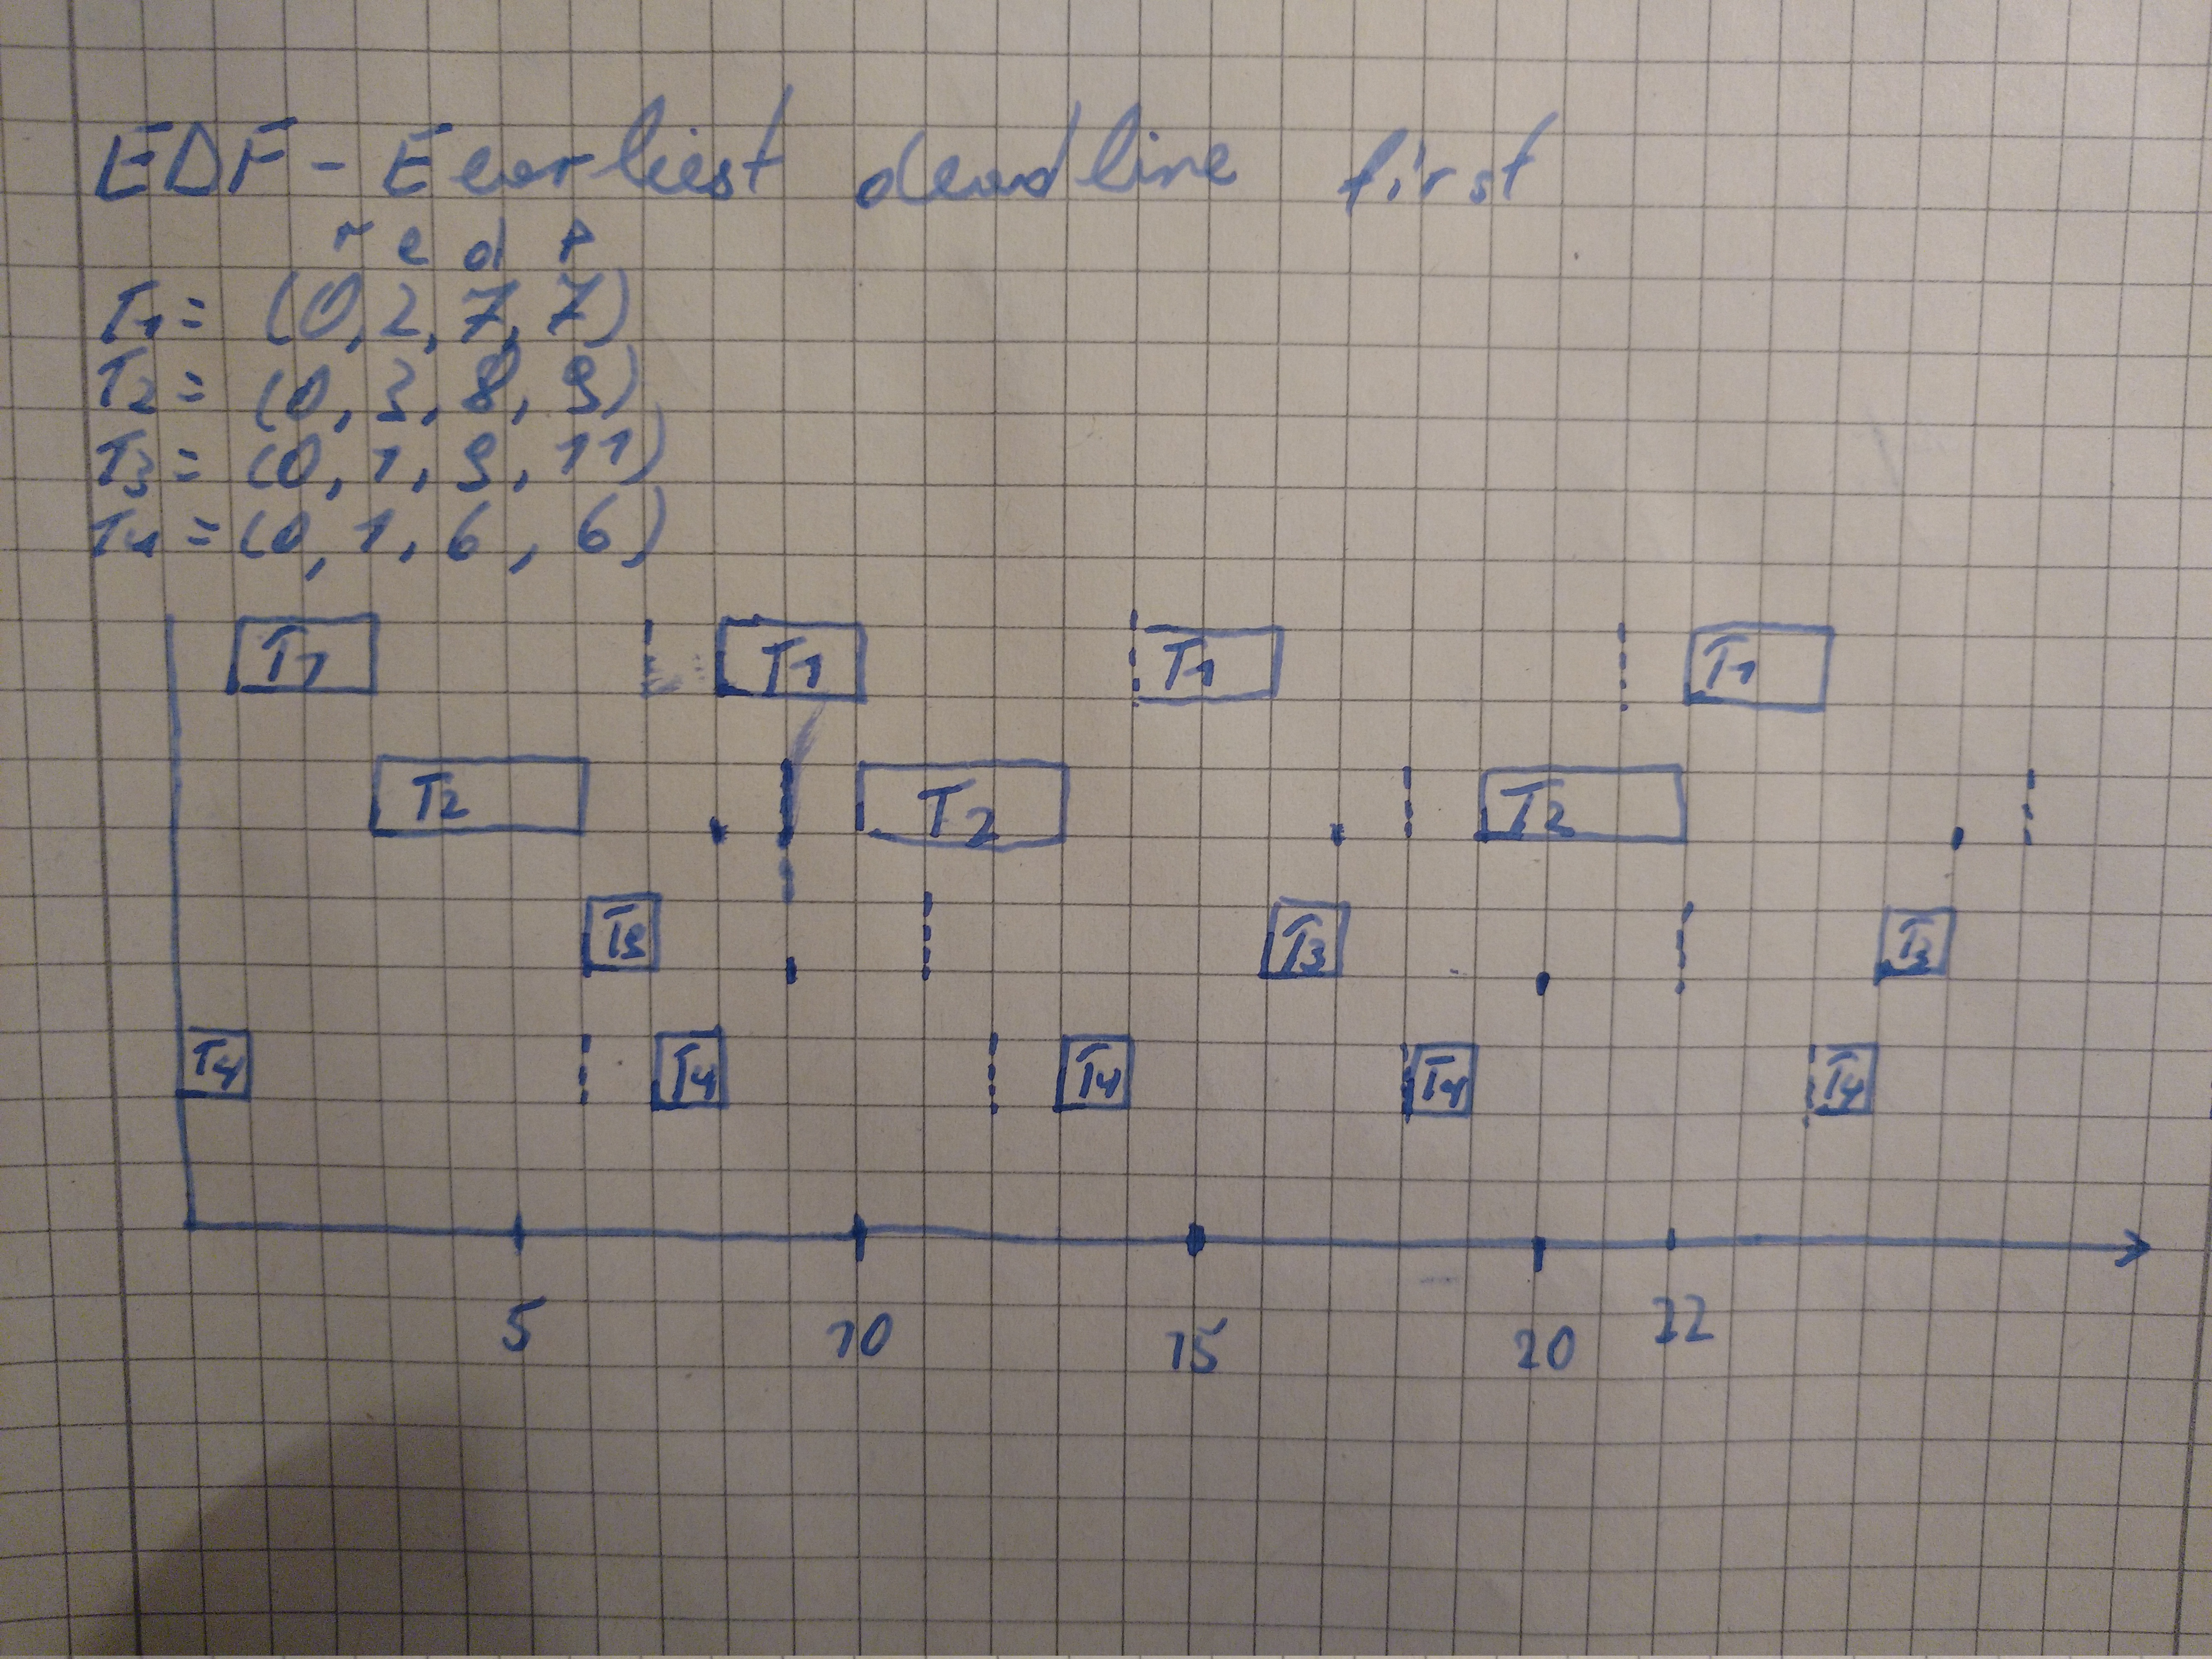
\includegraphics[width=\textwidth]{./exercise3/EDF.jpg} \clearpage
\item[d)] LLF \\
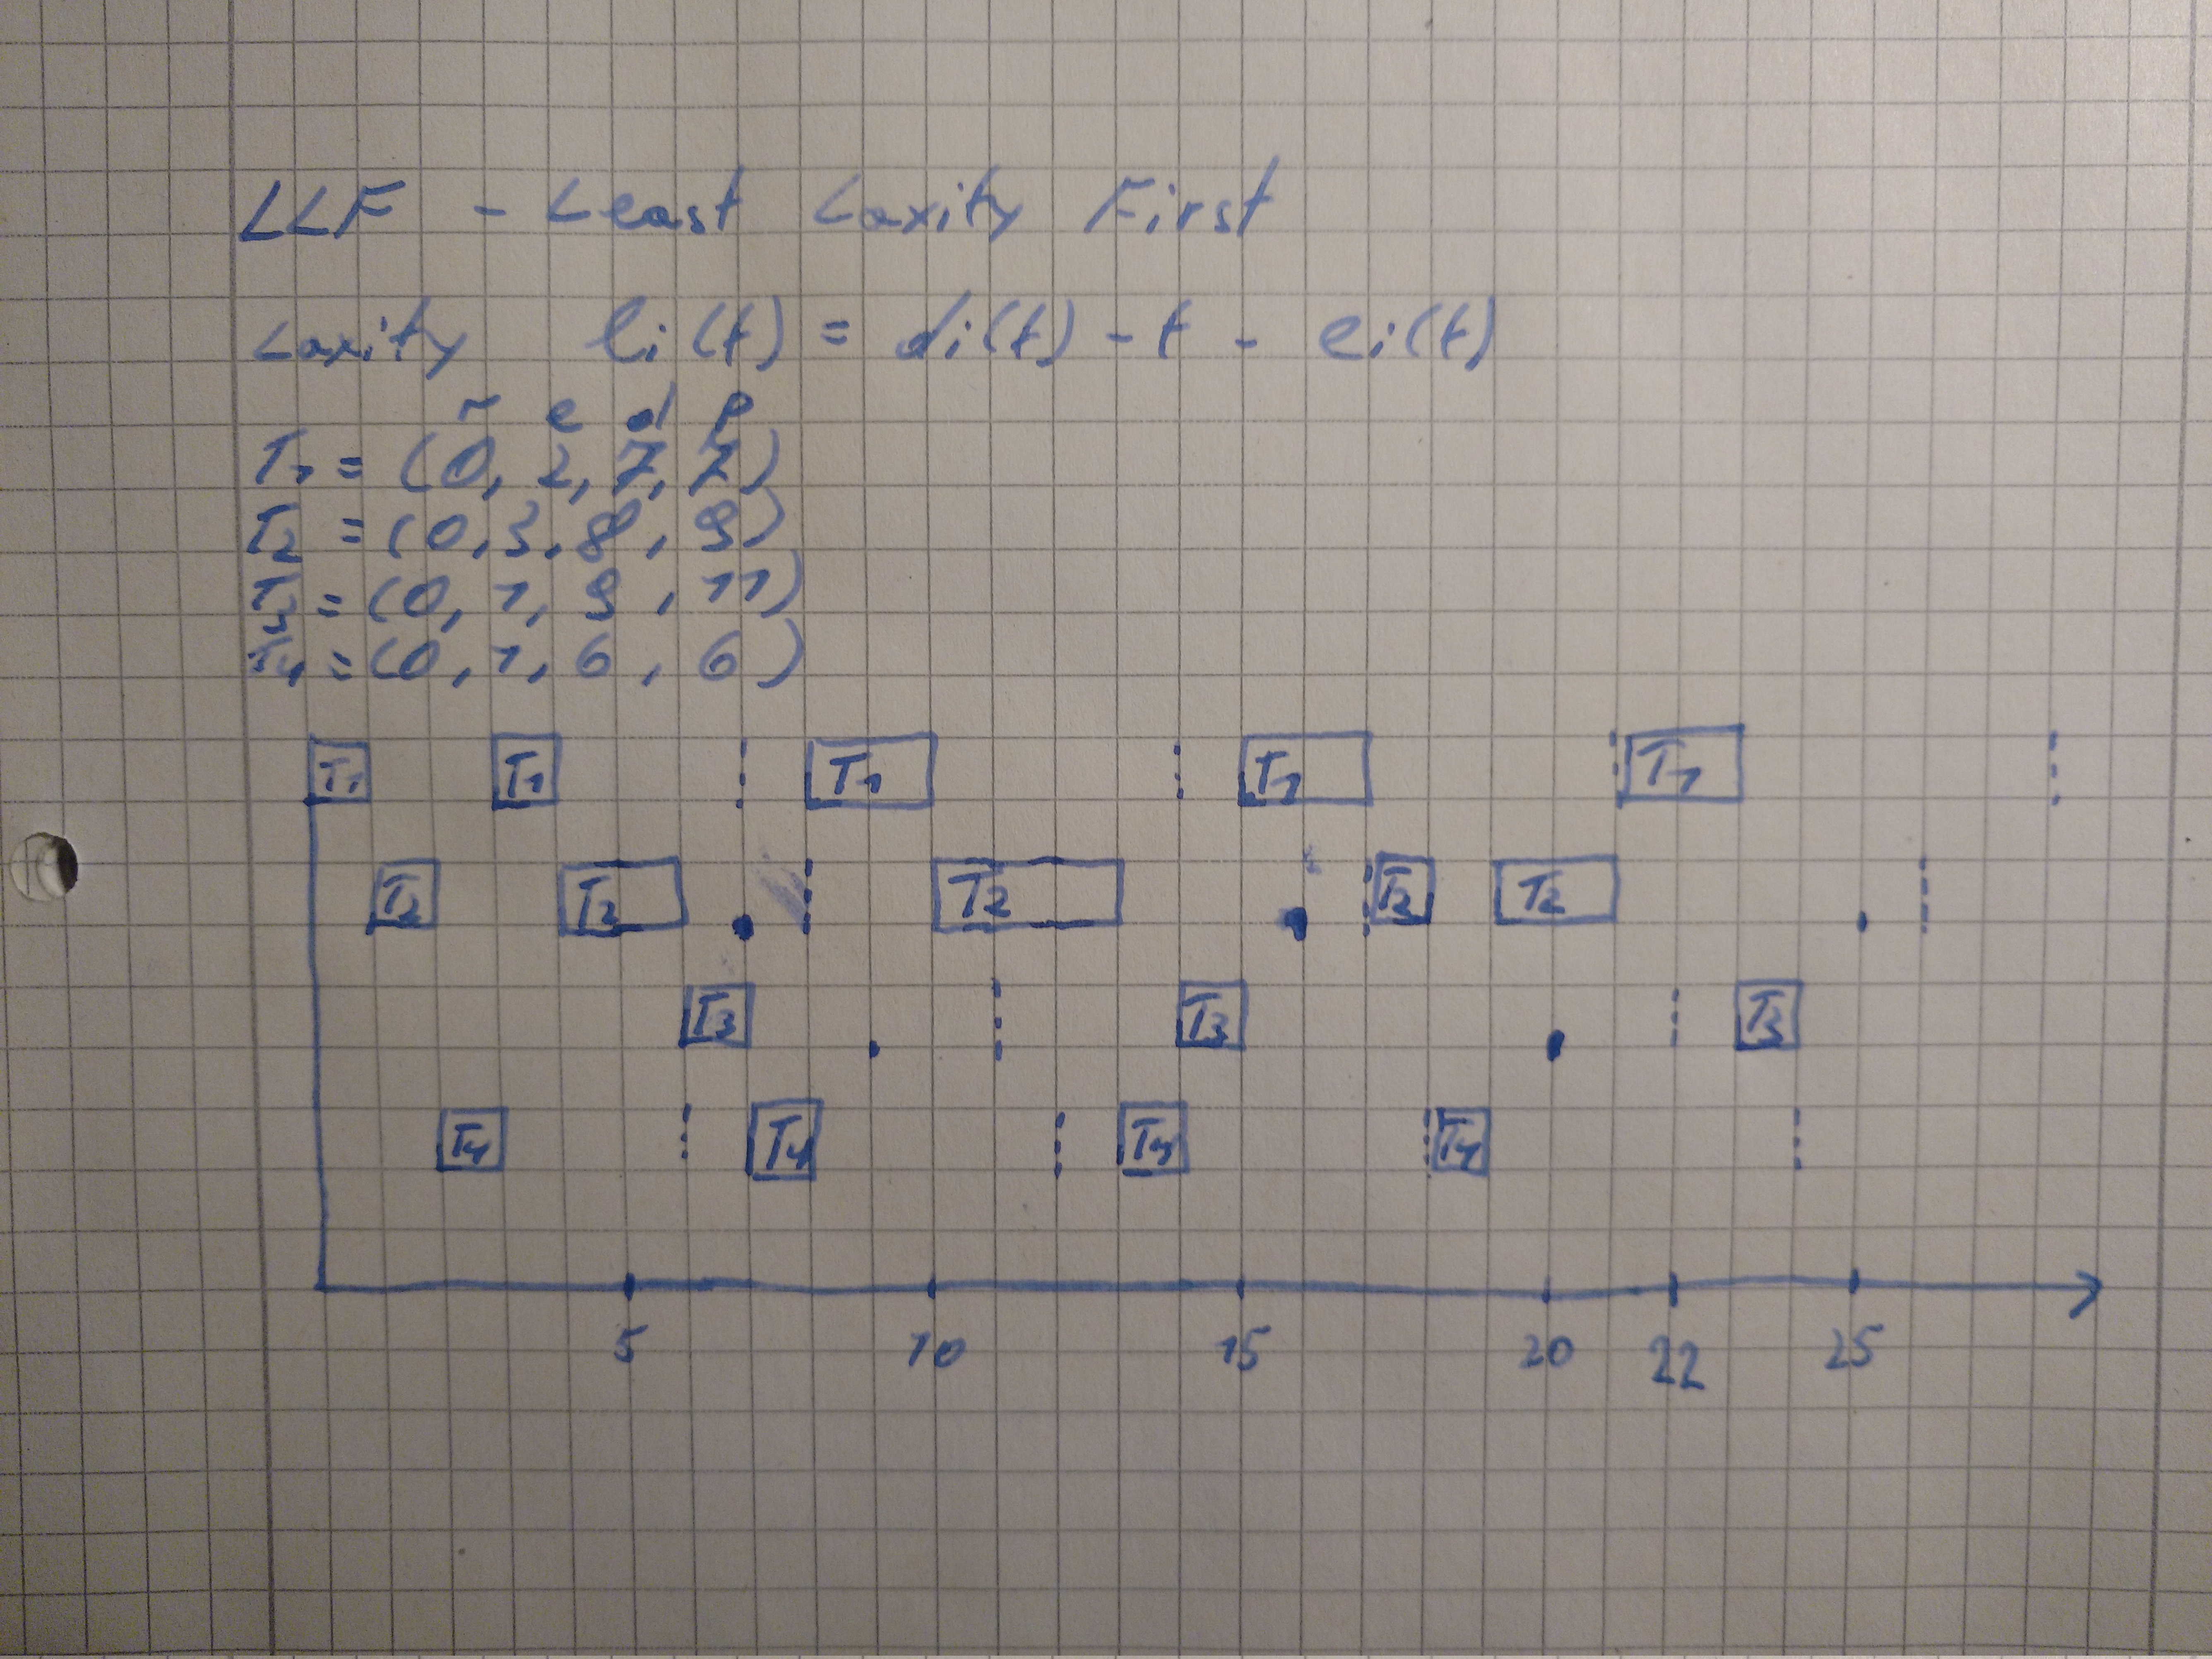
\includegraphics[width=\textwidth]{./exercise3/LLF.jpg} 

\end{enumerate}

\section*{4. Aufgabe}
Ja, das System ist realisierbar. In einer Sekunde gibt es 1000 Millisekunden, deswegen müssen wir ein Bild je $\frac{1000}{25} = 40$ Millisekunden fertig kriegen. Wir könne mit dem LLF Algorithmus das Problem leicht lösen. Wenn man die Zeit in 5-Millisekunden-Abschnitte zerteilt, wird in der ersten Millisekunde die Sprachverbindung bearbeitet und in den restlichen 4 die Bildbearbeitung. So schafft man die ganze Bildbearbeitung in 5 solche Abschnitte (20ms Bearbeitung) und verpasst dadurch keine Sprachverbindung. Das ganze ist aber nur unter der Annahme möglich, dass LLF kleines Overhead hat, was leider nicht der Fall ist. Da es aber um ein weiches Echtzeitsystem geht, können wir es immer realisieren, in dem die Qualität vermindert wird.

\section*{5. Aufgabe}

% /////////////////////// END DOKUMENT /////////////////////////
\end{document}